\chapter{Experimentos e resultados}
\label{chap:Experimentos e resultados}
\lettrine{N}{este} capítulo presentaranse os experimentos realizados e os resultados obtidos.
Para iso, comezarase presentando unha vista xeral do proceso de experimentación, 
seguido dos propios experimentos realizados, para 
Finalmente analizar os resultados obtidos en conxunto e as conclusións que se poden extraer deles.

\section{Vista Xeral}
\label{sec:Vista Xeral}

definiciones generales?

O obxetivo do traballo é determinar se as redes implícitas son aptas para a tarefa de rexistro de retinas.
Aínda tomando o traballo de IDIR como punto de partida, a tarefa de rexistro de retinas é substancialmente diferente á de pulmóns, polo que non podemos asumir que os parámetros utilizados nese caso sexan os óptimos para este.

A principal comparación que estamos a realizar ao longo de todos os experimentos é sobre a función de activación utilizada (SIREN ou ReLU).
Debido ao gran espazo de búsqueda que implica probar todas as configuracións posibles, 
os experimentos iniciais cetraránse en fixar unha unha seria de parámetros con valores razonables para poder experimentar só con aqueles que podan ter un impacto máis significativo.

Ademais, debido ás diferencias entre as funcións de activación, cada unha require unha configuración diferente para obter os mellores resultados.
Por exemplo, SIREN tende a requerir de dun learning rate mais baixo que ReLU, presumiblemente debido a unha maior sensibilidade aos valores de inicialización e inesabilidade.
probar?

\section{Experimentos}
\label{sec:Experimentos}

\subsection{Experimentos iniciais}
\label{subsec:Experimentos iniciais}

Inicialmente tentaremos determinar uns valores aceptables algúns dos parámetros da rede, para poder centrarnos en experimentar con aqueles que teñen un impacto máis significativo posteriormente.
Isto é relevante xa que moitos destes parámetros son dependentes uns de outros (por exemplo, a resolución utilizada inflúe no tamaño do batch size que se pode utilizar).

\subsubsection{Función de loss}
\label{subsubsec:Función de loss}

\paragraph{Planteamento}
\label{par:Planteamento}

A función de loss é un dos aspectos máis importantes á hora de entrenar unha rede neuronal.
Entre as funcións de loss valoradas para este traballo, que xa forón explicadas en \ref{subsubsec:Termos de loss}, atopamos:

\begin{itemize}
    \item MSE (Mean Squared Error)
    \item Huber
    \item Smooth L1
    \item NCC (Normalized Cross-Correlation)
    \item SSIM (Structural Similarity Index)
\end{itemize}


\paragraph{Resultados}
\label{par:Resultados}



\paragraph{Discusión}
\label{par:Discusión}

Aquelas métricas que non teñen en conta a estructura da imaxe (MSE, Huber, Smooth L1) non son ideais xa que é común que existan diferenzas de iluminación ou contraste entre a imaxe fixa e a imaxe móbil.
Por outro lado, NCC e SSIM son máis robustas a estas diferenzas xa que teñen en conta a estructura da imaxe, polo que son mais preferibles.

NCC é mais robusta a combios uniformes na intensidade global, mentres que SSIM é mais robusta a cambios locais a custo dun maior custo computacional e maior sensibilidade a ruido e o tamaño das seccións.

\paragraph{Conclusións}
\label{par:Conclusións}

\subsubsection{Resolución da imaxe}
\label{subsubsec:Resolución da imaxe}

\paragraph{Planteamento}
\label{par:Planteamento}

A resolución da imaxe é un aspecto clave xa que inflúe de forma directa no resto de parámetros da rede.
Por exemplo, un batch size de 1000 puntos nunha imaxe de 256x256 é unha densidade de puntos moito maior que nunha imaxe de 512x512.

Ademais, a resolución da imaxe tamén inflúe na capacidade da rede para aprender as transformacións, xa que a información que recibe é mais detallada. 
Isto pode ser beneficioso se estos detalles conteñen información relevante para a tarefa de rexistro, pero tamén podería ser perxudicial se conteñen unha gran parte de ruido.

O tamaño das imaxes tamén é unha das principais diferencias entre as imaxes de retina e as de pulmóns utilizadas orixinalmente por IDIR, tendo estas últimas de 512x512 e as primeiras de ata 2160x2160.

Para determinar cal é a resolución mais adecuada, realizáronse experimentos comparando o rendemento de cada unha sobre unha mostra de imaxes dos datases de FIRE e RFMID.
Debido a que a rede non é capaz de rexistrar con éxito a gran parte das imaxes, tomaráse a distancia media de todos os puntos como métrica de comparación.

\paragraph{Resultados}
\label{par:Resultados}

\begin{table}[h]
    \centering
    \begin{minipage}[t]{0.45\linewidth}
        \centering
        \begin{tabular}{|c|c|}
        \hline
        Resolution & Mean Distance \\ \hline
        250 & 251.29 \\ \hline
        750 & 250.62 \\ \hline
        1250 & 250.59 \\ \hline
        1708 & 250.59 \\ \hline
        \end{tabular}
        \caption{Mean Distances for MLP (FIRE)}
        \label{tab:mlp_mean_distances_fire}
    \end{minipage}
    \hfill
    \begin{minipage}[t]{0.45\linewidth}
        \centering
        \begin{tabular}{|c|c|}
        \hline
        Resolution & Mean Distance \\ \hline
        250 & 263.85 \\ \hline
        750 & 263.19 \\ \hline
        1250 & 258.56 \\ \hline
        1708 & 258.06 \\ \hline
        \end{tabular}
        \caption{Mean Distances for SIREN (FIRE)}
        \label{tab:siren_mean_distances_fire}
    \end{minipage}
\end{table}

\begin{table}[h]
    \centering
    \begin{minipage}[t]{0.45\linewidth}
        \centering
        \begin{tabular}{|c|c|}
        \hline
        Resolution & Mean Distance \\ \hline
        250 & 36.18 \\ \hline
        750 & 36.01 \\ \hline
        1250 & 36.03 \\ \hline
        1708 & 36.04 \\ \hline
        \end{tabular}
        \caption{Mean Distances for MLP (RFMID)}
        \label{tab:mlp_mean_distances_rfmid}
    \end{minipage}
    \hfill
    \begin{minipage}[t]{0.45\linewidth}
        \centering
        \begin{tabular}{|c|c|}
        \hline
        Resolution & Mean Distance \\ \hline
        250 & 73.42 \\ \hline
        750 & 77.55 \\ \hline
        1250 & 67.33 \\ \hline
        1708 & 67.31 \\ \hline
        \end{tabular}
        \caption{Mean Distances for SIREN (RFMID)}
        \label{tab:siren_mean_distances_rfmid}
    \end{minipage}
\end{table}

\paragraph{Discusión}
\label{par:Discusión}

Pódese observar como unha maior resolución tende a dar mellores resultados, pero a un custo computacional maior.

\paragraph{Conclusións}
\label{par:Conclusións}

Poderís ser interesante determinar cal é o punto de inflexión onde o aumento da resolución non compensa o aumento do rendemento.

\subsubsection{Regularización}
\label{subsubsec:Regularización}

\paragraph{Planteamento}
\label{par:Planteamento}

O proceso de regularización axuda a rede a evitar o sobreaxuste, modificando o termo de loss para penalizar as transformacións pouco realistas.
Entre as técnicas de regularización valoradas para este traballo, que xa forón explicadas en \ref{subsubsec:Regularización}, atopamos:

\begin{itemize}
    \item Jacobian regularizer
    \item Hyperelastic regularizer
    \item Bending energy penalty
\end{itemize}

Se os termos de regularización son demasiado grandes, a rede fará transformacións moi pequenas para evitar ser penalizada, o que resulta nunha transformación insuficiente.
Por outro lado, se os termos son demasiado pequenos, a rede fará transformacións moi grandes, o que resulta nunha transformación irrealista e sobreaxustada.
A cantidade óptima de regularización depende da parexa concreta de imaxes a alinear, polo que intentaremos determinar cal é a mellor para unha mostra de imaxes ...

\paragraph{Resultados}
\label{par:Resultados}

\paragraph{Discusión}
\label{par:Discusión}

\paragraph{Conclusións}
\label{par:Conclusións}



\subsubsection{Learning rate}
\label{subsubsec:Learning rate}

\paragraph{Planteamento}
\label{par:Planteamento}

Debido á natureza da rede, o batch size utilzado ten unha relación directa co batch size, polo que tentaremos determinar a relación óptima entre ambos.
Ao igual que os experimentos anteriores, esta norma pode ser diferente para cada función de activación, polo que realizaremos experimentos separados para cada unha.

\paragraph{Resultados}
\label{par:Resultados}

\paragraph{Discusión}
\label{par:Discusión}

\paragraph{Conclusións}
\label{par:Conclusións}


\subsection{Batch size}
\label{subsec:Batch size}

Ao longo dos experimentos realizados, o análisis cualitativo revelou que o batch size é un dos parámetros que máis impacto ten no rendemento da rede.
Unha vez determinados uns valores aceptables nos parámetros anteriores, realizáronse experimentos para determinar cal era o batch size óptimo.

Obsérvase que un maior batch size tende a dar mellores resultados, pero a un custo computacional maior. Interesa determinar cal é o punto de inflexión onde o aumento do batch size non compensa o aumento do rendemento.

Divídense os datasets en FIRE categoría S e RFMID por dificultade xa que testean cousas diferentes

\subsection{Estratexias de mostraxe}
\label{subsec:Estratexias de mostraxe}

Orixinalmente IDIR utiliza unha estratexia de mostraxe aleatoria para seleccionar os puntos que se pasan á rede en cada iteración.
Mentres que esta estretexia parece suficiente para o rexitro de pulmóns, no caso das imaxes de retina isto non ten porque ser así.
Isto debe a que as imaxes de retina teñen seccións con moita mais información que outras, frente os CTs de pulmóns que está moita mais repartida.
Ademais, teñen maiores desprazamentos e menor superposición entre cada parella. 

Para solucionar isto, propúxose unha estratexia de mostraxe mais intellixente, onde se calcula unha máscara de probabilidade para cada imaxe, que se utiliza para seleccionar os puntos que se pasan á rede.
Para calcular esta máscara, extráense mediante operadores de Sobel os vasos sanguíneos e mediante umbralización o disco óptico, que son as zonas onde se espera que haxa máis información, e dáselles mais probabilidades de ser seleccionadas.
Esta aproximación estaba errada, \dots

Posteriormente probouse unha estratexia de mostraxe uniforme, onde se seleccionan un número fixo de puntos en cada imaxe, independentemente da información que conteña.
É unha estratexia similar ao mostraxe aleatorio, pero garantindo que se cubre a maior parte posible da imaxe. Isto é importante en experimentos con batch sizes pequenos.
A implementación non foi moi sinxela xa que repartir uniformemente un número arbitrario de puntos dentro duncha máscara circular (mais non perfectamente circular) non é tan trivial como repartilos nunha máscara rectangular.

Así mesmo implementouse un scheduling do batch size, coa intención de utilizar poucos puntos inicialmente para que a rede aprenda a transformación global, e aumentar o número de puntos conforme avanzase o entrenamento para que a rede aprenda as transformación locais.

\begin{figure}[]
    \centering
    \begin{subfigure}[b]{0.3\textwidth}
        \centering
        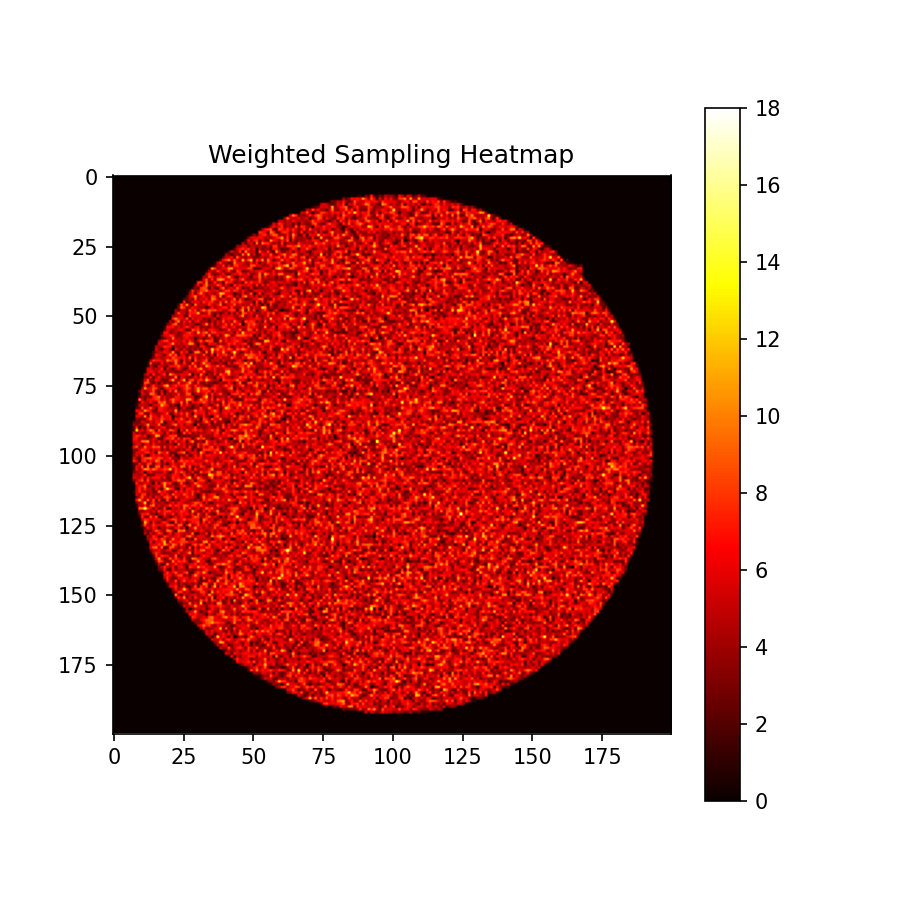
\includegraphics[width=\textwidth]{imaxes/random_sampling_heatmap.png}
        \caption{Heatmap de mostraxe aleatorio}
        \label{fig:random_sampling_heatmap}
    \end{subfigure}
    \hfill
    \begin{subfigure}[b]{0.3\textwidth}
        \centering
        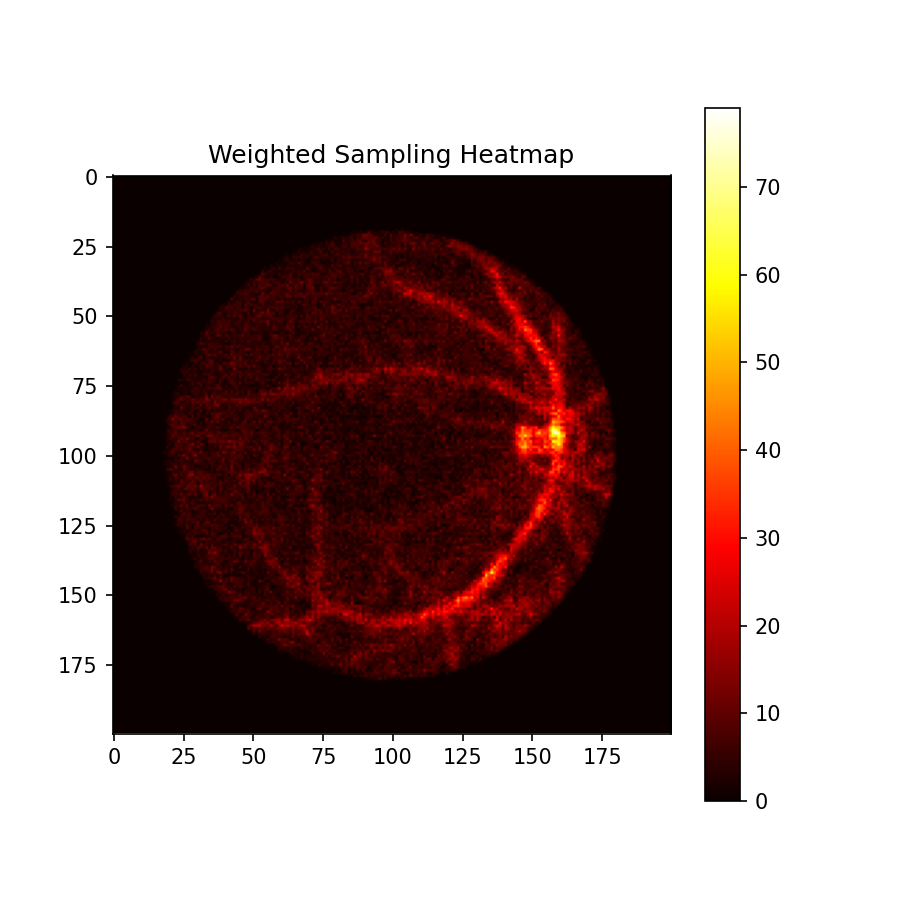
\includegraphics[width=\textwidth]{imaxes/weighted_sampling_heatmap.png}
        \caption{Heatmap de mostraxe con peso}
        \label{fig:weighted_sampling_heatmap}
    \end{subfigure}
    \hfill
    \begin{subfigure}[b]{0.3\textwidth}
        \centering
        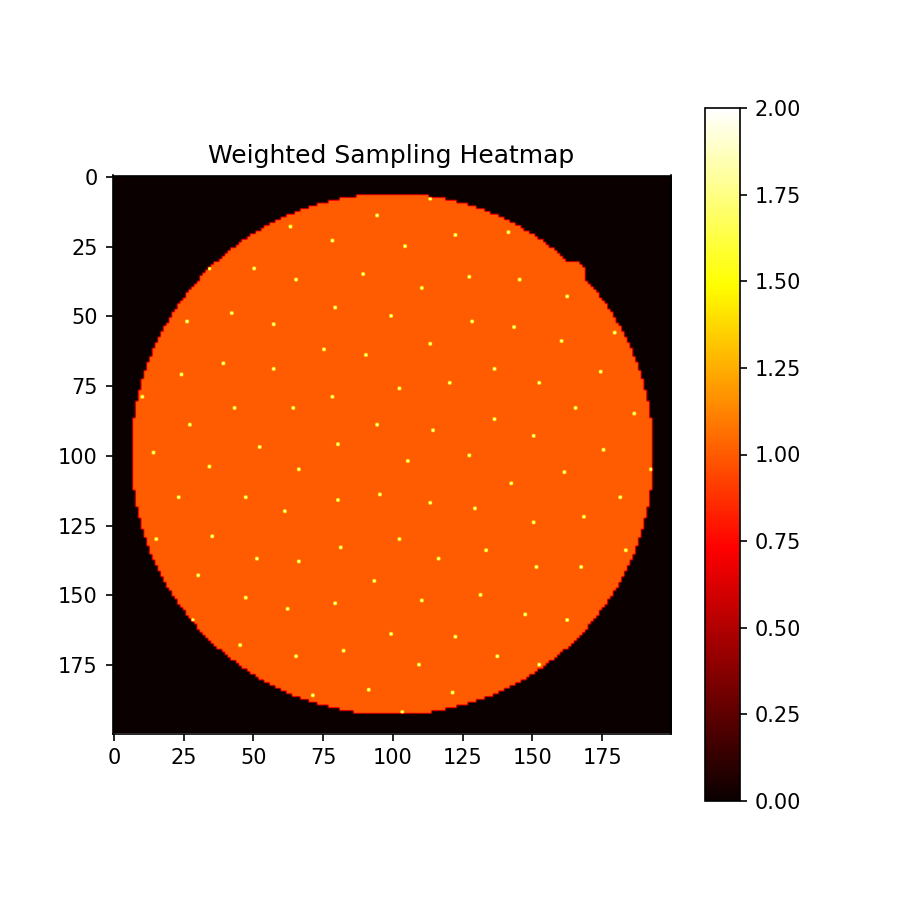
\includegraphics[width=\textwidth]{imaxes/uniform_sampling_heatmap.png}
        \caption{Heatmap de mostraxe uniforme (100 puntos)}
        \label{fig:uniform_sampling_heatmap}
    \end{subfigure}
    \caption{Heatmaps de mostraxe}
    \label{fig:sampling_heatmaps}
\end{figure}


Parece que non tén un impacto significativo no rendemento da rede, polo que se decidiu manter a estratexia de mostraxe aleatoria.

\subsection{Inicialización}
\label{subsec:Inicialización}

É posible que a inicialización da rede sexa un factor mais importante que a estratexia de mostraxe\dots

Implementouse unha lotería de inicialización, onde se utiliza o loss no epoch 0 para determinar a inicialización da rede mais beneficiosa.
É posible que fore mellor esperar ata un epoch algo mais avanzado para determinar a inicialización, xa que no epoch 0 non hay ningunha seguridade de que non sexa un mínimo local.